\ProvidesFile{ch2.tex}[]

\chapter{Uncertainty-aware localization microscopy by variational diffusion}
\ix{physics//Physics appendix}

\section{Introduction}

\subsection{The curse of dimensionality}

Dimensionality refers to the number of variables or features in a dataset. In conventional fluorescence nanoscopy, an image generated by (1.1) containing $M$ fluorophores has $2M$ parameters. Similarly, the image itself is a high dimensional variable where the number of pixels is the number of dimensions. As the number of dimensions in the parameter space increases, it becomes increasingly difficult to infer the parameters from the data. The curse of dimensionality is a term coined to describe various phenomena that arise when working with high-dimensional data, making statistical analysis and machine learning more challenging. Mathematically, the curse of dimensionality can be described through the following issues.

As dimensionality increases, the volume of the space grows exponentially. For instance, the volume of a hypercube with side length $l$ in $d$-dimensional space is given by $l^d$. This rapid increase in volume means that data points become sparser, making it difficult to estimate densities and find meaningful patterns. Furthermore, in high-dimensional spaces, the concept of distance becomes less informative. The difference between the minimum and maximum distance between data points tends to shrink as dimensionality increases, which can make clustering and nearest-neighbor algorithms less effective. With a large number of dimensions, models can easily become overly complex, capturing noise instead of the underlying signal. This leads to overfitting, where the model performs well on training data but poorly on unseen data.

Deep models have captured the attention of many researchers, as they can perform inference tasks in high dimensional spaces without an excessive computational burden. These models are not entirely immune to the curse of dimensionality or the complexity of data distributions, however, and overfitting is still an important problem. Simultaneously, many deep models are deterministic neural networks, which give a single output given an input. This is in sharp contrast to classical statistical inference methodologies such as Bayesian inference, which model a distribution on their outputs, allowing one to express uncertainties during inference. Bayesian methods such as Markov Chain Monte Carlo (MCMC) or variational inference lack the scaling of deep learning but maintain a scientific value \parencite{Kingma2013}.

\subsection{The Bayesian calculation}

Bayesian inference provides a rigorous framework for updating beliefs about the world in light of new data. It leverages the principles of probability theory to combine prior knowledge with empirical evidence, resulting in updated, posterior beliefs. In parametric modeling, we assume that the data $x$ are generated from a distribution with a set of parameters $y$. Parametric models simplify the problem by assuming a specific form for the underlying distribution of the data, characterized by a finite set of parameters. This approach allows us to use mathematical functions to describe complex systems and make inferences about the parameters based on observed data.

At the heart of Bayesian inference is Bayes' rule, which allows us to update our beliefs based on new evidence. Bayes' rule is derived from the definition of conditional probability. The conditional probability of $y$ given $x$ is defined as $p(y \lvert x) = \frac{p(x,y)}{p(y)}$ provided that $p(y) > 0$. Similarly, the conditional probability of $x$ given $y$ is $p(x \lvert y) = \frac{p(x,y)}{p(x)}$. Rearranging these equations and solving for $p(y\lvert x)$ gives us Bayes' rule:

\begin{equation*}
p(y \lvert x) = \frac{p(x \lvert y) p(y)}{p(x)}.
\end{equation*}

Here, $p(y \lvert x)$ is the called the posterior distribution, representing our updated beliefs about the parameters after observing the data. $p(x \lvert y)$ is the likelihood, the probability of the observed data given the parameters. $p(y)$ is the prior distribution, representing our beliefs about the parameters before observing the data. $p(x)$ is the marginal likelihood or evidence, which normalizes the posterior distribution and ensures it sums to one.

One of the main challenges in Bayesian inference is the computation of the posterior distribution. The denominator in Bayes' rule, $p(x)$, involves an integral over all possible values of the parameters:

\begin{equation*}
p(x) = \int p(x \lvert y) p(y) \, dy.
\end{equation*}

In many practical applications, this integral is intractable due to the high dimensionality of the parameter space. To address this challenge, various approximation methods have been developed. One such method is Markov Chain Monte Carlo (MCMC), which generates samples from the posterior distribution by constructing a Markov chain that has the desired distribution as its equilibrium distribution. MCMC algorithms were originally developed for applications in statistical physics but were eventually adapted to a broader range of statistical problems. Well known MCMC algorithms include the Metropolis-Hastings algoritm, Gibbs sampler \parencite{Geman1984}, and gradient-based algorithms inspired by Langevin dynamics. In general, MCMC is asymptotically exact but can be computationally expensive for large datasets and high dimensional parameter spaces. Variational inference is an alternative approach, which is not exact, but reduces the computational burden in these scenarios.

\subsection{Variational inference}

Variational inference involves approximating the true posterior distribution \( q(y \lvert x) \) with a simpler, parameterized distribution \( p_{\psi}(y) \) by minimizing the Kullback-Leibler (KL) divergence between them. The KL divergence \( D_{KL}(q(y \lvert x) \lvert\lvert p_{\psi}(y)) \) measures how one probability distribution diverges from a second probability distribution. To minimize the KL divergence, we first express it as

\begin{equation*}
D_{KL}(q(y \lvert x) \lvert\lvert p_{\psi}(y)) = \mathbb{E}_{q(y \lvert x)}\left[\log \frac{q(y \lvert x)}{p_{\psi}(y)}\right]
\end{equation*}

This can be rewritten using Bayes' rule as

\begin{align*}
D_{KL}(q(y \lvert x) \lvert\lvert p_{\psi}(y\lvert x)) &= \mathbb{E}_{q(y \lvert x)}\left[\log \frac{q(y \lvert x)}{p_{\psi}(y\lvert x)}\right] \\
&= \mathbb{E}_{q(y \lvert x)}\left[\log \frac{q(y\lvert x)p_{\psi}(x)}{p_{\psi}(x,y)} \right]\\
&= \mathbb{E}_{q(y \lvert x)}\left[\log \frac{q(y\lvert x)}{p_{\psi}(x,y)} \right] + \mathbb{E}_{q(y \lvert x)}\left[\log p_{\psi}(x) \right]
\end{align*}

Defining $\mathcal{L} = -\mathbb{E}_{q(y \lvert x)}\left[\log \frac{q(y\lvert x)}{p_{\psi}(x,y)} \right]  = \mathbb{E}_{q(y \lvert x)}\left[\log \frac{p_{\psi}(x,y)}{q(y\lvert x)} \right] $, we can write,

\begin{equation*}
\mathbb{E}_{q(y \lvert x)}\left[\log p_{\psi}(x) \right] = D_{KL}(q(y \lvert x) \lvert\lvert p_{\psi}(y\lvert x)) + \mathcal{L} \geq \mathcal{L}
\end{equation*}

which is often called a variational objective. Given that \( \log p_{\psi}(x) \) is constant, minimizing $D_{KL}(q(y \lvert x) \lvert\lvert p_{\psi}(y\lvert x))$ is equivalent to maximizing $\mathcal{L}$. For practical reasons, we often instead solve a minimization problem with respect to $\psi$

\begin{equation*}
\mathbb{E}_{q(y \lvert x)}\left[-\log p_{\psi}(x) \right] \leq -\mathcal{L} = \mathbb{E}_{q(y \lvert x)}\left[-\log \frac{p_{\psi}(x,y)}{q(y\lvert x)} \right]
\end{equation*}

This approach provides a practical way to perform Bayesian inference, especially in high-dimensional settings. It is worth noting that this derivation often begins with $D_{KL}(p_{\psi}(y\lvert x) \lvert\lvert q(y \lvert x) ) $ such that the expectation is taken with respect to the model distribution, since the true distribution is unknown. However, for the following application, the target distribution is known and thus the objective is prudently formulated in this way. 


\subsection{A note on variational inference for functions}

For some applications, we would like to perform inference when the mapping between latents and observed data is deterministic. For example, there might be a determinisitic mapping $f$ between high resolution images and low-resolution ones, and we want to infer the high resolution image from the low resolution image. In that case, we find

\begin{align*}
\mathbb{E}_{q(y \lvert x)}\left[-\log p_{\psi}(x) \right] &\leq \mathbb{E}_{q(y \lvert x)}\left[-\log \frac{p_{\psi}(x,y)}{q(y\lvert x)} \right]\\
&= \mathbb{E}_{q(y \lvert x)}\left[-\log \frac{p_{\psi}(y)}{q(y\lvert x)} \right] + \mathbb{E}_{q(y \lvert x)}\left[-\log p_{\psi}(x\lvert y) \right] \\
&= \mathbb{E}_{q(y \lvert x)}\left[-\log \frac{p_{\psi}(y)}{q(y\lvert x)} \right] + \mathbb{E}_{q(y \lvert x)}\left[-\log \delta(x-f(y)) \right] 
\end{align*}

The second term is to be safely neglected, as it is undefined and provides no meaningful information during optimization. 

\subsection{Blending Bayesian inference with deep models for microscopy}

Deep models have attracted tremendous attention from researchers in the natural sciences, with several foundational applications arising in microscopy \parencite{Weigert2018,Falk2019}. Recently, the application of deep image translation in nanoscopy has received considerable interest. Recently, the use of deep models to perform localization has been proposed as an alternative to traditional localization algorithms, in order to increase imaging speed and labeling density. In previous applications of deep models to localization microscopy, super-resolution images have been recovered from a sparse set of localizations with conditional generative adversarial networks \parencite{Ouyang2018} or localization itself can be performed using traditional convolutional networks \parencite{Nehme2020,Speiser2021}. Here, we perform localization indirectly by predicting kernel density (KD) estimates of a population of fluorescent molecules using a deep model. 

Kernel density estimation in nanoscopy is necessarily performed using a single low-resolution image, and thus common measures of model performance are based on localization errors computed over ensembles of simulated images. Unfortunately, this choice precludes computation of uncertainty at test time under a fixed model. Bayesian probability theory is therefore an attractive alternative, which offers us mathematically grounded tools to reason about uncertainty. 

We model a posterior on high-resolution KD estimates conditioned on a low-resolution image. Our approach is based on a type of score based generative model \parencite{Song2021}, referred to as a denoising diffusion probabilistic model (DDPM) in the literature \parencite{Ho2020,Song2021}. We find that this technique is complementary to relevant existing approaches to uncertainty estimation, which would primarily address epistemic sources of uncertainty, using techniques such as ensembling \parencite{Lakshminarayanan2017} or Monte Carlo dropout \parencite{Gal2022}. The approach is inspired by recent variational perspectives on diffusion \parencite{Dirmeier2023,Ribeiro2024,Kingma2021,Kingma2023}.  Such techniques provide a mechanism for scalable variational inference, which can be trained using a variational bound written in terms of the signal-to-noise ratio of the diffused data, and a simple noise estimation loss. Indeed, recent efforts have shown that the variational bound can be reparameterized to give several more conventional diffusion losses \parencite{Kingma2021,Kingma2023,Ribeiro2024}. 

In the remainder of this chapter, we introduce KD estimation as an alternative to direct localization using low-resolution images, followed by demonstration of our variational diffusion model for measuring uncertainty estimation at scale. 

\section{Results}

We now consider datasets $(\bold{x}_i,\bold{y}_{0,i},\hat{\bold{y}}_{i})_{i=1}^{N}$ of observed images $\bold{x}_i$ true KD images $\bold{y}_{0,i}$, and augmented low-resolution inputs $\hat{\bold{y}}_{i}=\phi(\bold{x}_{i})$, where $\phi$ is a convolutional neural network (CNN).

\subsection{Approach}

Direct optimization of the image likelihood from observations $\bold{x}$ alone is challenging when fluorescent emitters are dense within the field of view and fluorescent signals significantly overlap. However, CNNs have recently proven to be powerful tools fluorescence microscopy to extract parameters describing fluorescent emitters such as color, emitter orientation, $z$-coordinate, and background signal \cite{Zhang2018,Kim2019,Zelger2018}. For localization tasks, CNNs typically employ upsampling layers to reconstruct Bernoulli probabilities of emitter occupancy \parencite{Speiser2021,Nehme2020}. We choose to instead infer KDEs, denoted by $\bold{y}$, which are latent in the low-resolution data $\bold{x}$. KDEs are a common data structure used in nanoscopy, and can be easily generated from molecular coordinates, alongside observations $\bold{x}$.

To go beyond point estimation of the KDE given the low-resolution data, we seek a generative model for the posterior. Unfortunately, the posterior can be intractable, since molecules cannot be easily resolved and therefore its dimensionality is not well-defined. To address this issue, we instead model a conditional distribution on the latent $\bold{y}$: $p(\bold{y}\lvert\bold{x})$, where $\bold{y}$ is of known dimensionality. We choose to model $p(\bold{y}\lvert\bold{x})$ with a diffusion model, given that the distribution $p(\bold{y}\lvert\bold{x})$ is expensive to compute.

Sampling from diffusion models can be computationally expensive, given that generation amounts to solving a complex stochastic differential equation, effectively mapping a simple base distribution to the complex data distribution. The solution of such equations requires numerical integration with very small step sizes, resulting in thousands of neural network evaluations \parencite{Saharia2021,Vahdat2021}. For conditional generation tasks in high-risk applications, generation complexity is further exacerbated by the need for the highest level of detail in generated samples. Therefore, we propose that sampling is preceded by an augmentation network $\phi$, which in essence generates an initial estimate to guide the diffusion process. Reasoning for this choice in our application is two-fold:

\textbf{Synthesis Speed}. By training the augmentation network $\phi$ to obtain an approximate estimate of the KDE, we can reduce the number of iterations, since the diffusion model only needs to model the remaining mismatch, resulting in a less complex model from which sampling becomes easier. Speed is critical in SMLM applications, which can produce thousands of images in a single experiment.

\textbf{Sample Fidelity}. Since diffusion will often be initialized in low-density regions of the data distribution, inaccurate score estimation in these regions will negatively affect the sampling process. Moreover, mixing can be difficult because of the need of traversing low density regions to transition between modes of the distribution \parencite{Song2019}.

\subsection{Variational diffusion}

Diffusion models \parencite{Ho2020,Song2021} are a class of generative models originally inspired by nonequilibrium statistical physics, which slowly destroy structure in a data distribution via a fixed Markov chain referred to as the \emph{forward process}. In the present context, we leverage the variational interpretation of this model class \parencite{Kingma2021,Kingma2023} to approximate the posterior $p(\bold{y}\lvert\bold{x})$. 

\textbf{Diffusion Model}. We use a forward process which gradually adds Gaussian noise to the latent $\bold{y}_0$ in discrete time, according to a variance schedule $\beta_{t}$:

\begin{equation}
q(\bold{y}_{T}\lvert\bold{y}_{0}) = \prod_{t=1}^{T}q(\bold{y}_{t}\lvert\bold{y}_{t-1}) \;\;\; q(\bold{y}_{t}\lvert\bold{y}_{t-1}) = \mathcal{N}\left(\sqrt{1-\beta_{t}}\bold{y}_{t-1},\beta_t I\right)
\end{equation}


\clearpage
\begin{figure}
    \centering
    \begin{tikzpicture}[thick,scale=1.5, every node/.style={scale=1.5}]
        % Original Graphical Model
        \node[obs] (x) {$\mathbf{y}_0$};
        \node[latent, right=45pt of x] (z1) {$\mathbf{y}_1$};
        \node[latent, right=45pt of z1] (z2) {$\mathbf{y}_{2}$};
        \draw node[draw=none, scale=0.8, right=9pt of z2] (z3) {\rotatebox{0}{$\mathbf{\cdots}$}};
        \node[latent, right=22.5pt of z3] (zt) {$\mathbf{y}_T$};
        \edge[-{Latex[scale=1.0]}]{x}{z1}
        \node[rectangle, draw=none, fill=white, scale=0.66, right=2.25pt of x, yshift=9pt] (eq1) {};
        \node[rectangle, draw=none, fill=white, scale=0.66, right=2.25pt of z1, yshift=9pt] (eq2) {};
        \node[rectangle, draw=none, fill=white, scale=0.66, below=-0.27pt of z3] (eq3) {};
        
        \edge[-{Latex[scale=1.0]}]{z1}{z2}
        \node[rectangle, draw=none, scale=0.66, above=22.5pt of zt] (nt) {$\mathcal{N}\big(0, \beta_{T}\mathbf{I}\big)$};
        \node[rectangle, draw=none, scale=0.66, above=22.5pt of z2] (n2) {$\mathcal{N}\big(0, \beta_{2}\mathbf{I}\big)$};
        \node[rectangle, draw=none, scale=0.66, above=22.5pt of z1] (n1) {$\mathcal{N}\big(0, \beta_{1}\mathbf{I}\big)$};
        \edge[-{Latex[scale=1.0]}]{nt}{zt}
        \edge[-{Latex[scale=1.0]}]{n2}{z2}
        \edge[-{Latex[scale=1.0]}]{n1}{z1}

        \edge[-]{z2}{z3}
        \edge[-{Latex[scale=1.0]}]{z3}{zt}

        \node[obs, below=40pt of x] (x2) {$\mathbf{y}_0$};
        \node[latent, right=45pt of x2] (z1_2) {$\mathbf{y}_1$};
        \node[latent, right=45pt of z1_2] (z2_2) {$\mathbf{y}_{2}$};
        \draw node[draw=none, scale=0.8, right=9pt of z2_2] (z3_2) {\rotatebox{0}{$\mathbf{\cdots}$}};
        \node[latent, right=22.5pt of z3_2] (zt_2) {$\mathbf{y}_T$};

        \edge[-{Latex[scale=1.0]}]{z1_2}{x2}
        \node[rectangle, draw=none, fill=white, scale=0.66, right=2.25pt of x2, yshift=9pt] (eq1_2) {};
        \node[rectangle, draw=none, fill=white, scale=0.66, right=2.25pt of z1_2, yshift=9pt] (eq2_2) {};
        \node[rectangle, draw=none, fill=white, scale=0.66, below=-0.27pt of z3_2] (eq3_2) {};

        \edge[-{Latex[scale=1.0]}]{z2_2}{z1_2}
        \edge[-]{zt_2}{z3_2}
        \edge[-{Latex[scale=1.0]}]{z3_2}{z2_2}
    \end{tikzpicture}
    \caption{\textbf{Diffusion model with Markovian transitions}. The forward process (top) is a Markovian Gaussian diffusion process of $\bold{y}$ with variance schedule $\beta_{t}$. The reverse process (bottom) conditionally generates $\bold{y}$ from noise}
    \label{fig:fig10}
\end{figure}


\begin{figure}
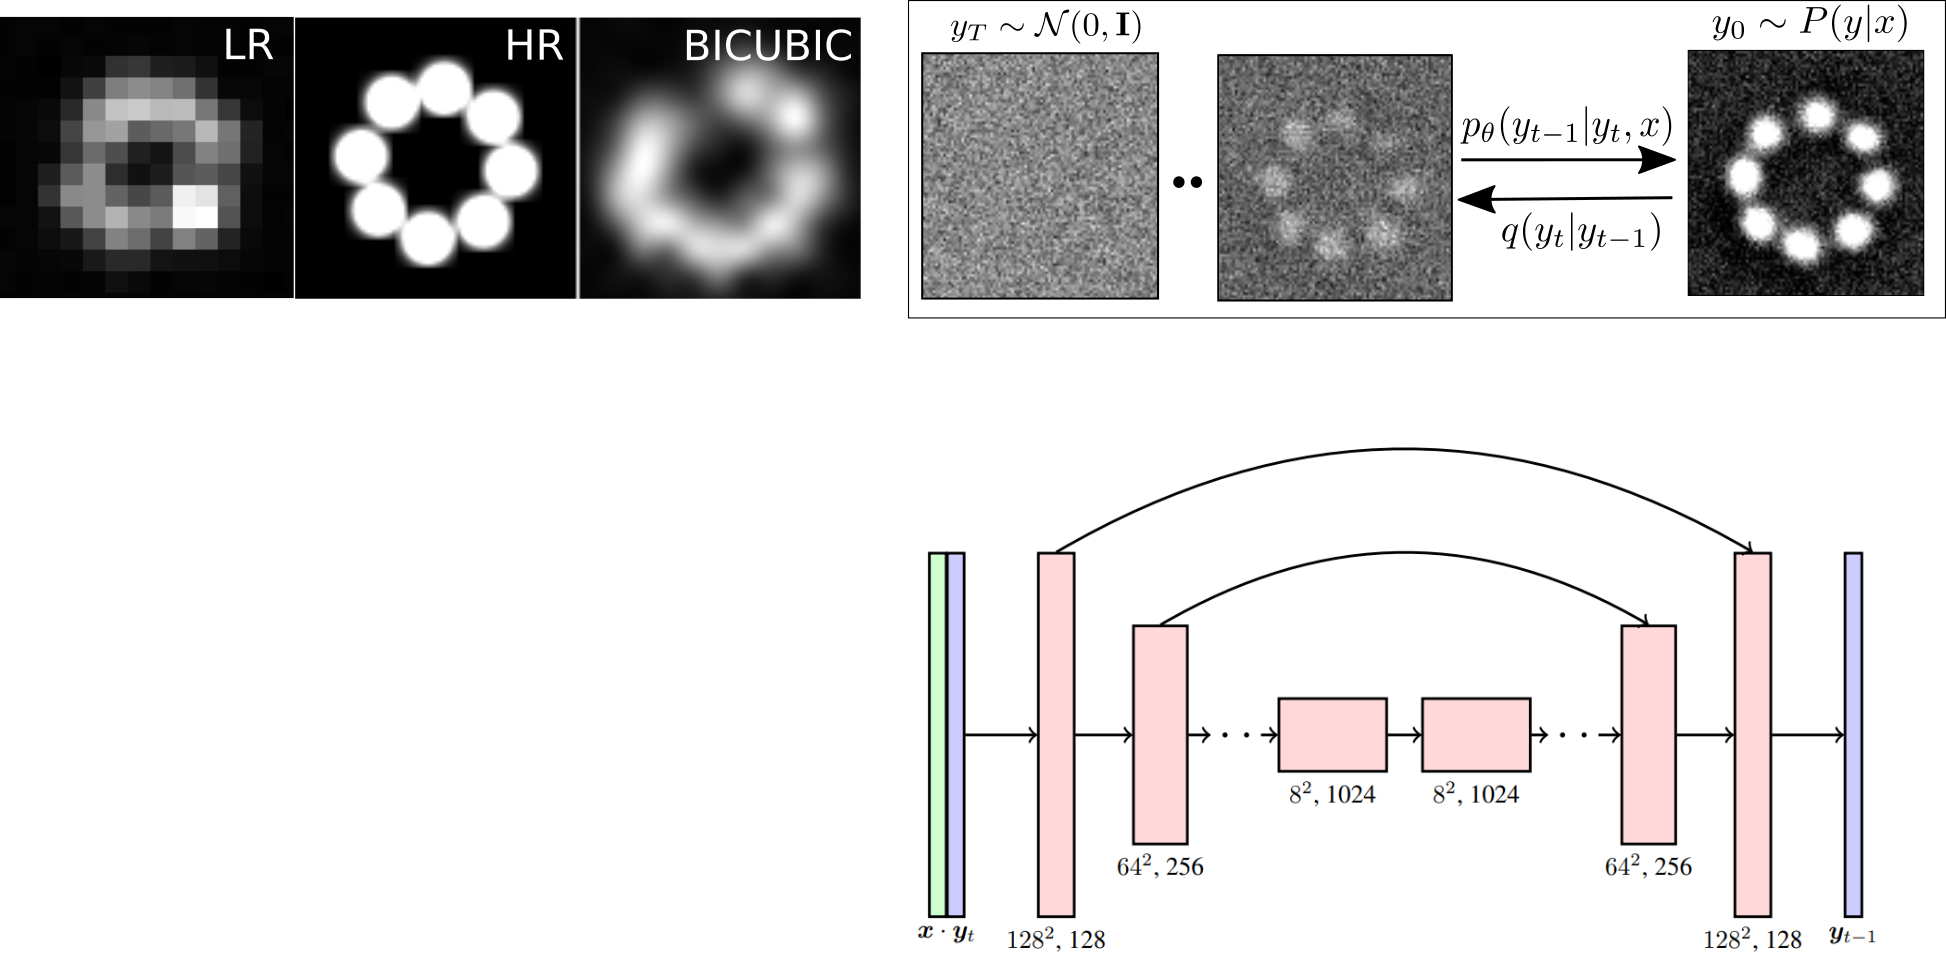
\includegraphics[scale=0.5]{/Users/cwseitz/git/cwseitz.github.io/docs/phd/ddpm/ddpm/media/Diffusion.png}
\caption{\textbf{Uncertainty estimation by variational diffusion}. Example diffusion process of the latent high resolution image $\bold{y}$ conditioned on the low resolution image $\bold{x}$. The terminal $\bold{y}_{0}$ represents a sample from $p(\bold{y}\lvert\bold{x})$.}
\label{fig:fig11}
\end{figure}

An important property of the forward process is that it admits sampling $\bold{y}_t$ at an arbitrary timestep $t$ in closed form \parencite{Ho2020}. Using the notation $\alpha_t := 1 - \beta_t$ and $\gamma_t := \prod_{s=1}^{t} \alpha_s$, we have $q(\bold{y}_t\lvert\bold{y}_0) = \mathcal{N} \left(\sqrt{\gamma_{t}} \bold{y}_{0}, (1 - \gamma_t)I \right)$ or $\bold{y}_{t} = \sqrt{\gamma_{t}}\bold{y}_{0} + \sqrt{1-\gamma_{t}}\bold{\epsilon}$ for $\epsilon \sim \mathcal{N}(0,I)$. The signal to noise ratio (SNR) as defined in \parencite{Kingma2023}, at a time step $t$ reads $\mathrm{SNR}_t = \gamma_{t}/(1-\gamma_{t})$.

The usual procedure is then to learn a parametric representation of the \emph{reverse process}, and therefore generate samples of the latent $\bold{y}_{0}$ from  $p(\bold{y}_{0}\lvert\bold{x})$. Formally, $p_{\psi}(\bold{y}_{0}\lvert\bold{x}) = \int p_{\psi}(\bold{y}_{0:T}\lvert\bold{x})d\bold{y}_{1:T}$ where $\bold{y}_{t}$ is a latent representation with the same dimensionality of the data and $p_{\psi}(\bold{y}_{0:T}\lvert\bold{x})$ is a Markov process, starting from a noise sample $p_{\psi}(\bold{y}_{T}) = \mathcal{N}(0,I)$. Writing this Markov process gives

\begin{equation}
p_{\psi}(\bold{y}_{0:T}\lvert\bold{x}) = p_{\psi}(\bold{y}_{T})\prod_{t=1}^{T} p_{\psi}(\bold{y}_{t-1}\lvert\bold{y}_{t},\bold{x}) \;\;\; p_{\psi}(\bold{y}_{t-1}\lvert\bold{y}_{t},\bold{x}) = \mathcal{N}\left(\mu_{\psi}(\bold{y}_{t},\gamma_{t}),\beta_{t}I\right)
\end{equation}

where we reuse the variance schedule of the forward process \parencite{Ho2020}. From (5) it can be seen that the learnable parameter in the reverse process is the expectation of the transition $\mu_{\psi}$ where $\psi$ is a neural network. 

Learning the reverse process can be approached by either regressing noise $\bold{\epsilon}$ from the forward process, or the true latent $\bold{y}_{0}$, as there is a deterministic relationship between them. We adopt the former for consistency with other work, and define $\psi$ as a neural denoising function which regresses the noise $\bold{\epsilon}$ from a noisy $\bold{y}_{t}$. A relation between the noise estimate $\epsilon_{\psi}$ and $\mu_{\psi}$ is given in the Appendix, which gives an intuition for sampling. The proposed sampling scheme is depicted in (Figure \ref{fig:fig11}). 

\textbf{Variational Objective}. Following \parencite{Kingma2021}, we interpret the reverse process as a hierarchical generative model that samples a sequence of latents $\bold{y}_{t}$, with time running backward. Training of the model is achieved through the variational bound

\begin{align}
-\log p(\bold{y}_{0}) &\leq -\mathbb{E}_{q(\bold{y}_{1:T}\lvert\bold{y}_{0})} \log \left(\frac{p_{\psi}(\bold{y}_{1:T},\bold{y}_{0})}{q(\bold{y}_{1:T}\lvert\bold{y}_{0})}\right) \\
&=  D_{KL}(q(\bold{y}_{T}\lvert\bold{y}_{0}) \lvert\lvert p(\bold{y}_{T})) + \mathbb{E}_{q(\bold{y}_{1}\lvert\bold{y}_{0})} \log p(\bold{y}_{0}\lvert\bold{y}_{1}) + \mathcal{L}_{\psi}
\end{align}

where we have omitted conditioning on the low-resolution $\bold{x}$ to simplify the notation. Note that, this is similar to a hierarchical VAE, but in a diffusion model $q(\bold{y}_{1:T}\lvert\bold{y}_{0})$ is fixed by the forward process rather than learned. The so-called diffusion loss $\mathcal{L}_{\psi}$ is shown in the Appendix, and is the term of interest as the first two terms do not contribute meaningfully to the loss \parencite{Ho2020}. Furthermore, it has become standard to use simplified forms of $\mathcal{L}_{\psi}$, such as a noise estimation loss, as this has shown superior performance. Importantly, $\mathcal{L}_{\psi}$ is simply a reweighted variant of a family of diffusion objectives \parencite{Kingma2021,Kingma2023}. We use the following Monte Carlo estimate of $\mathcal{L}_{\psi}$, which demonstrates that the variational bound can be written in terms of the common noise-estimation loss


\begin{equation}
\mathcal{L}_{\psi} = \mathbb{E}_{\epsilon\sim \mathcal{N}(0,I),t\sim U(1,T)}\left[\left(\frac{\mathrm{SNR}_{t-1}}{{\mathrm{SNR}_{t}}}-1\right)\lvert\lvert \bold{\epsilon}-\bold{\epsilon}_{\psi}\lvert\lvert_{2}^{2}\right]
\end{equation}

A full derivation of this objective is outlined in the Appendix. Note that $\mathrm{SNR}_{t}$ is monotonically decreasing with $t$, and thus $\frac{\mathrm{SNR}_{t-1}}{{\mathrm{SNR}_{t}}} = \frac{\gamma_{t-1}}{\gamma_{t}}\frac{1-\gamma_{t}}{1-\gamma_{t-1}} \geq 1$, ensuring $\mathcal{L}_{\psi}\geq 0$. In this paper, we choose to use a uniformly weighted loss and leave the exploration of the weighted loss to future work.

\subsection{Experiments}

All training data consits of low-resolution $20\times 20$ images, setting $\sigma_{\bold{x}}=0.92$ in units of low-resolution pixels, for consistency with common experimental conditions with a 60x magnification objective lens and numerical aperture (NA) of 1.4. We multiply $\omega_{k}$ by a constant $i_{0}=200$ for experiments for consistency with typical fluorophore emission rates. All KDEs have dimension $80\times 80$, are scaled between $[0,1]$, and are generated using $\sigma_{\bold{y}}=3.0$ pixels in the upsampled image (Figure \ref{fig:fig12}). For a typical CMOS camera, this results in KDE pixels with lateral dimension of $\approx 27\mathrm{nm}$. Initial coordinates $\theta$ were drawn uniformly over a two-dimensional disc with a radius of 7 low-resolution pixels.


\begin{figure}
\centering
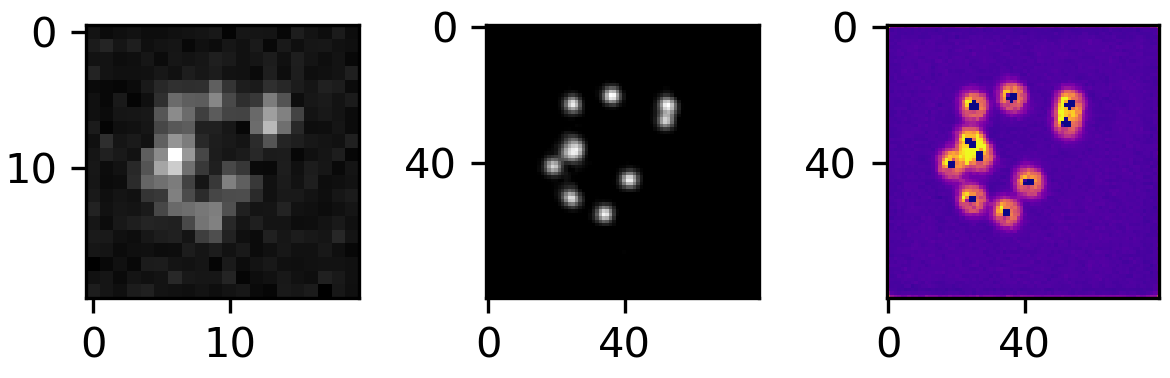
\includegraphics[scale=1.1]{/Users/cwseitz/git/cwseitz.github.io/docs/phd/ddpm/ddpm/media/Bayes.png}
\caption{\textbf{Non cherry-picked estimation of marginal variances}. A low-resolution image $\bold{x}$ (left column) is transformed by $\phi$ to produce a KDE estimate $\hat{\bold{y}}$ (middle column) and a DDPM $\psi$ computes a map of marginal variances (right column)}
\label{fig:fig12}
\end{figure}

\textbf{Localization RMSE}. In order to verify the initial predictions made by the augmentation model $\phi$, we simulated a dataset $(\bold{x}_i,\bold{y}_{0,i},\hat{\bold{y}}_{i})_{i=1}^{N}$ with $N=1000$. Objects in the KDE $\hat{\bold{y}}_{i}$  are detected using the Laplacian of Gaussian (LoG) detection algorithm \parencite{Kong2013}, which permits more direct comparison of model predictions to the Cramer-Rao lower bound on localization error, compared to other image similarity measures (Figure \ref{fig:fig15}). Localization is carried out from scale-space maxima directly in LoG, as opposed to fitting a model function to KDEs. A particular LoG localization in the KDE is paired to the nearest ground truth localization and is unpaired if a localization is not within 5 KDE pixels of any ground truth localization. In addition to localization error, we measure a precision $\mathrm{P = TP/(TP + FP)} = 1.0$ and recall $\mathrm{R = TP/(TP + FN)} = 0.85$, where $\mathrm{TP}$ denotes true positive localizations, $\mathrm{FP}$ denotes false positive localizations, and $\mathrm{FN}$ denotes false negative localizations.


\textbf{Variational Diffusion}. We set $T = 100$ for all experiments and treat forward process variances $\beta_{t}$ as hyperparameters, with a linear schedule from $\beta_{0}=10^{-4}$ to $\beta_{T}=10^{-2}$.
These constants were chosen to be small relative to ground truth KDEs, which are scaled to $[-1,1]$, ensuring that forward process distribution $\bold{y}_{T}\sim q(\bold{y}_{T}\lvert\bold{y}_{0})$ approximately matches the reverse process $\bold{y}_T\sim \mathcal{N}(0, I)$ at $t=T$. Example KD estimates from low-resolution images and the marginal variances obtained from sampling $N=100$ samples from $p_{\psi}(\bold{y}_{0}\lvert\bold{x})$ are shown in (Figure 4). 


\section{Conclusion}

We proposed a variational diffusion model for uncertainty-aware localization microscopy. Our approach builds on recent advancements in conditional diffusion models, to model the posterior distribution on high-resolution KD estimates from low-resolution inputs. This tractable posterior distribution is constructed by first augmenting low resolution inputs to a KD estimate using the DeepSTORM architecture with minor modifications \parencite{Nehme2020}. Conditioning a diffusion model on this initial estimate permits sampling with relatively fewer samples than most existing diffusion models in similar applications, thereby making computation of marginal variances possible. Our approach made three core contributions: (i) we derived a relationship between the posterior on kernel density estimates with the posterior on molecular locations, and (ii) we demonstrated that a diffusion model can model a distribution on KDEs with qualitatively similar marginal variances expected from predictions made using MCMC. By using a recently discovered relationship of the variational lower bound to a traditional noise-estimation objective, we can confidently approximate the true posterior.

\section{Broader impact}

The development of a method for uncertainty estimation in super-resolution imaging, as proposed here, holds implications beyond its immediate application in SMLM. By leveraging diffusion models for uncertainty estimation, this approach not only enhances the reliability of super-resolution image reconstructions but also extends its utility to a diverse array of domains. The incorporation of a guided diffusion process facilitates efficient reconstruction while maintaining intepretation of the underlying uncertainty. Importantly, the principles underlying this method resonate across various fields, suggesting its potential applicability in domains beyond microscopy. For instance, the extension of similar techniques to general image processing tasks highlights the potential to address uncertainty in a wide range of applications in bioimaging or medical imaging. Moreover, the utilization of diffusion models for uncertainty estimation aligns with a broader trend in leveraging probabilistic frameworks for enhancing deep learning applications, with implications extending to fields such as natural language processing, computer vision, and autonomous systems. By bridging these interdisciplinary boundaries, this method not only addresses a critical need in localization microscopy but also contributes to the advancement of uncertainty-aware deep learning methodologies.


\section{Appendix}

\subsection{Sampling}

Sampling from the reverse process $p_{\psi}(\bold{y}_{t-1}\lvert\bold{y}_{t},\bold{x})$ is achieved by estimation of the noise $\epsilon_{\psi}$ from $\bold{y}_{t}$ by the denoising model $\psi$, and therefore estimation of $\bold{y}_{0}$

\begin{equation}
\hat{\bold{y}}_{0} = \frac{1}{\sqrt{\gamma_{t}}}(\bold{y}_{t} - \sqrt{1-\gamma_{t}}\epsilon_{\psi})
\end{equation}

followed by sampling from the forward process $\bold{y}_{t-1} \sim q(\bold{y}_{t-1}\lvert\hat{\bold{y}}_{0}) = \mathcal{N}(\sqrt{\gamma_{t-1}},(1-\gamma_{t-1})I)$. 


\subsection{Derivation of the variational bound}

We now derive the so-called diffusion loss $\mathcal{L}_{\psi}$, written in (8) in the main text. Similar derivations can be found in \parencite{Kingma2021,Ribeiro2024}, and we include it here only for completeness

\begin{align*}
-\log p(\bold{y}_{0}) &\leq - \mathbb{E}_{q(\bold{y}_{1:T}\lvert\bold{y}_{0})} \log \frac{p(\bold{y}_{0:T})}{q(\bold{y}_{1:T}\lvert\bold{y}_{0})}\\
&= -\mathbb{E}_{q(\bold{y}_{1:T}\lvert\bold{y}_{0})} \log \frac{p(\bold{y}_{T})p(\bold{y}_0\lvert\bold{y}_1) \prod_{t=2}^{T}p(\bold{y}_{t-1}\lvert\bold{y}_t)}{q(\bold{y}_T\lvert\bold{y}_0)\prod_{t=2}^{T}q(\bold{y}_{t-1}\lvert\bold{y}_t,\bold{y}_0)}\\
&= -\mathbb{E}_{q(\bold{y}_{1:T}\lvert\bold{y}_{0})} \left[ p(\bold{y}_0\lvert\bold{y}_1) + \log \frac{p(\bold{y}_{T})}{q(\bold{y}_T\lvert\bold{y}_0)} + \sum_{t=2}^{T} \log \frac{p(\bold{y}_{t-1}\lvert\bold{y}_t)}{q(\bold{y}_{t-1}\lvert\bold{y}_t,\bold{y}_0)}\right]\\
&= -\mathbb{E}_{q(\bold{y}_{1:T}\lvert\bold{y}_{0})} \left[ p(\bold{y}_0\lvert\bold{y}_1)\right] + D_{KL}\left(q(\bold{y}_T\lvert\bold{y}_0) \lvert\lvert p(\bold{y}_{T})\right) \\
&+ \sum_{t=2}^{T} \mathbb{E}_{q(\bold{y}_{t}\lvert\bold{y}_{0})} D_{KL}\left(q(\bold{y}_{t-1}\lvert\bold{y}_t,\bold{y}_0)\lvert\lvert p(\bold{y}_{t-1}\lvert\bold{y}_t) \right)
\end{align*}

As before, we omit conditioning on $\bold{x}$ to simplify the notation. The first term is typically ignored, as it does not contribute meaningfully to the loss \parencite{Ribeiro2024}. Furthermore, the second term is approximately zero by construction. Therefore we are left with the last term, called the diffusion loss $\mathcal{L}_{\psi}$. The KL-divergence of $q$ and $p$ is between two Gaussians with identical variances $\sigma^{2} = \frac{(1-\gamma_{t-1})(1-\alpha_{t})}{1-\gamma_{t}}$, and expectations

\begin{align*}
\mu = \frac{\sqrt{\gamma_{t-1}}(1-\alpha_{t})}{1-\gamma_{t}}\bold{y}_{0}+ \frac{\sqrt{\alpha_{t}}(1-\gamma_{t-1})}{{1-\gamma_{t}}}\bold{y}_{t} \quad \mu_{\psi} = \frac{\sqrt{\gamma_{t-1}}(1-\alpha_{t})}{1-\gamma_{t}}\hat{\bold{y}}_{0}+ \frac{\sqrt{\alpha_{t}}(1-\gamma_{t-1})}{{1-\gamma_{t}}}\bold{y}_{t}
\end{align*}

for a fixed noise schedule \parencite{Saharia2021}. Therefore, we have

\begin{align*}
D_{KL}\left(q(\bold{y}_{t-1}\lvert\bold{y}_t,\bold{y}_0)\lvert\lvert p(\bold{y}_{t-1}\lvert\bold{y}_t) \right) &= \frac{1}{2\sigma^{2}} \lvert\lvert \mu - \mu_{\psi} \lvert\lvert_{2}^{2} \\
&= \frac{1}{2}\frac{\gamma_{t-1}(1-\alpha_{t})}{(1-\gamma_{t-1})(1-\gamma_{t})}\lvert\lvert \bold{y}_{0} - \hat{\bold{y}}_{0} \lvert\lvert_{2}^{2}\\
&= \frac{1}{2}\frac{\gamma_{t-1}((1-\gamma_{t})-\alpha_{t}(1-\gamma_{t-1}))}{(1-\gamma_{t-1})(1-\gamma_{t})}\lvert\lvert \bold{y}_{0} - \hat{\bold{y}}_{0} \lvert\lvert_{2}^{2}\\
&= \frac{1}{2}\frac{\gamma_{t-1}((1-\gamma_{t})-\frac{\gamma_{t}}{\gamma_{t-1}}(1-\gamma_{t-1}))}{(1-\gamma_{t-1})(1-\gamma_{t})}\lvert\lvert \bold{y}_{0} - \hat{\bold{y}}_{0} \lvert\lvert_{2}^{2}\\
&= \frac{1}{2}\left(\frac{\gamma_{t-1}}{1-\gamma_{t-1}}-\frac{\gamma_{t}}{1-\gamma_{t}}\right)\lvert\lvert \bold{y}_{0} - \hat{\bold{y}}_{0} \lvert\lvert_{2}^{2}\\
&= \frac{1}{2}\left(\mathrm{SNR}_{t-1}-\mathrm{SNR}_{t}\right)\lvert\lvert \bold{y}_{0} - \hat{\bold{y}}_{0} \lvert\lvert_{2}^{2}
\end{align*}

Reparameterizing the loss in terms of the noise, using $\lvert\lvert \bold{y}_{0} - \hat{\bold{y}}_{0} \lvert\lvert_{2}^{2} = \frac{1-\gamma_{t}}{\gamma_{t}}\lvert\lvert \bold{\epsilon}_{0} - \epsilon_{\psi} \lvert\lvert_{2}^{2}$ \parencite{Ribeiro2024}, we arrive at 

\begin{equation*}
\mathcal{L}_{\psi} = \frac{1}{2}\sum_{t=2}^{T} \mathbb{E}_{q(\bold{y}_{t}\lvert\bold{y}_{0})}\left(\frac{\mathrm{SNR}_{t-1}}{{\mathrm{SNR}_{t}}}-1\right)\lvert\lvert \bold{\epsilon}-\bold{\epsilon}_{\psi}\lvert\lvert_{2}^{2}
\end{equation*}

Using a Monte Carlo estimate of $\mathcal{L}_{\psi}$ \parencite{Kingma2023} which optimizes random terms of the summation to avoid calculating all terms simultaneously, we arrive at the objective written in the main text (8)

\begin{equation*}
\mathcal{L}_{\psi} = \mathbb{E}_{\epsilon\sim \mathcal{N}(0,I),t\sim U(1,T)}\left[\left(\frac{\mathrm{SNR}_{t-1}}{{\mathrm{SNR}_{t}}}-1\right)\lvert\lvert \bold{\epsilon}-\bold{\epsilon}_{\psi}\lvert\lvert_{2}^{2}\right]
\end{equation*}


\begin{figure}[t]
\centering
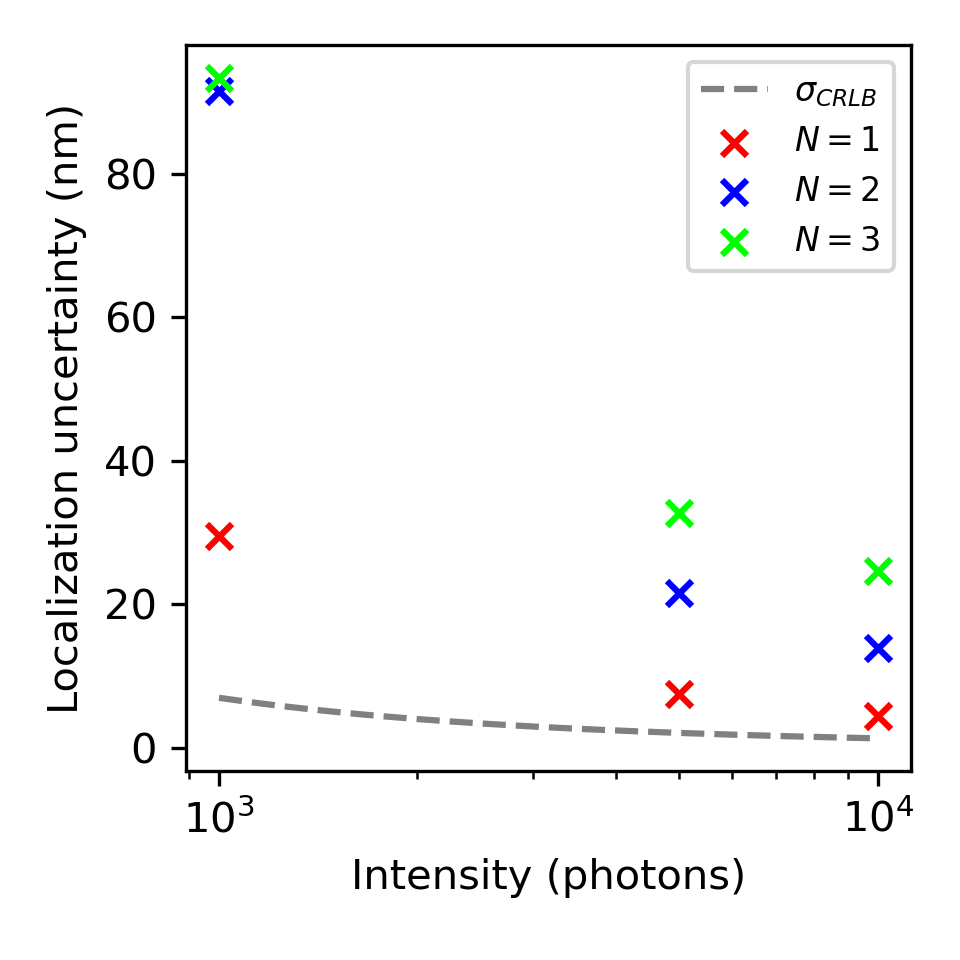
\includegraphics[scale=0.7]{/Users/cwseitz/git/cwseitz.github.io/docs/phd/ddpm/ddpm/media/Errors.png}
\caption{\textbf{Localization errors of the trained model $\phi$}. The Cramer-Rao lower bound is shown in red, computing by taking the diagonal elements of $I^{-1}(\theta)$.}
\label{fig:fig15}
\end{figure}


\subsection{Neural network architectures}

\begin{figure}[t]
\centering
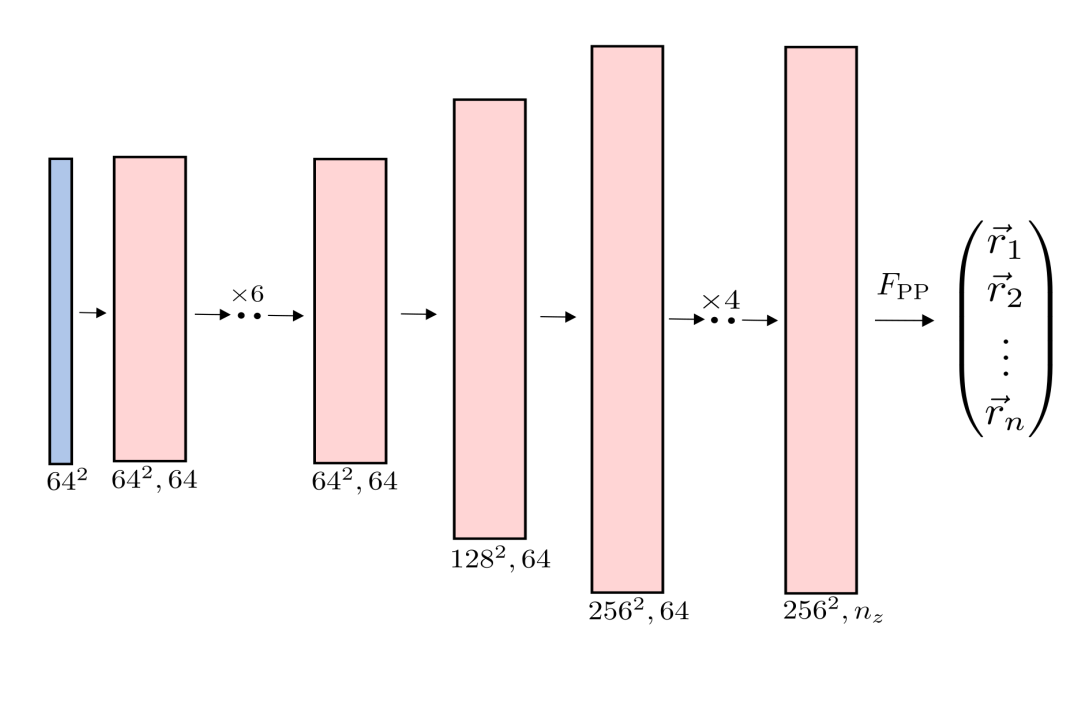
\includegraphics[scale=0.4]{/Users/cwseitz/git/cwseitz.github.io/docs/phd/ddpm/ddpm/media/DeepSTORM.png}
\caption{\textbf{Architecture of the augmenation model $\phi$}. A $20\times 20$ single-channel image is processed by eight convolutional blocks followed by a 4x upsampling module utilizing linear interpolation and a refinement module with six convolutional blocks. The number of output channels $n$ is set to one, but can be set to values greater than one to obtain axial resolution in three-dimensional localization microscopy}
\label{fig:fig13}
\end{figure}


\begin{figure}[t]
\centering
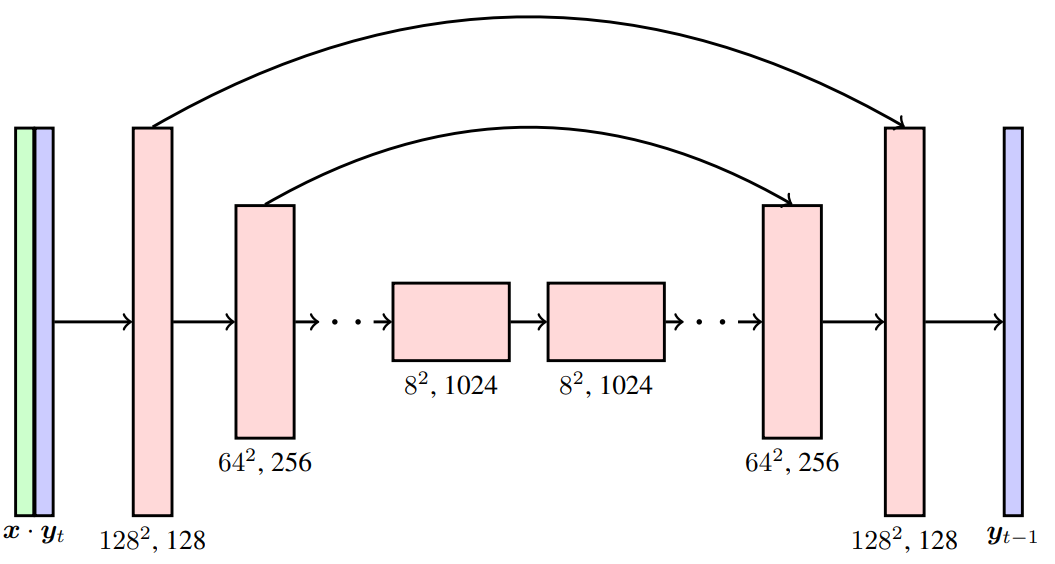
\includegraphics[scale=1.5]{/Users/cwseitz/git/cwseitz.github.io/docs/phd/ddpm/ddpm/media/DiffusionArch.png}
\caption{\textbf{Architecture of the denoising diffusion model}. A U-Net style architecture with channel multipliers of [1,2,4,8,16] downsamples and then upsamples the input image $\bold{y}_{t}$ to estimate $\bold{y}_{t-1}$}
\label{fig:fig14}
\end{figure}

\textbf{DeepSTORM CNN $\phi$}. The DeepSTORM CNN (Figure \ref{fig:fig13}), for 3D localization, can be viewed as a deep kernel density estimator, reconstructing kernel density estimates $\bold{y}$ from low-resolution inputs $\bold{x}$. We utilize a simplified form of the original architecture \parencite{Nehme2020} for 2D localization, which we denote $\phi$ in this paper, which consists of three main modules: a multi-scale context aggregation module, an upsampling module, and a prediction module. For context aggregation, the architecture utilizes dilated convolutions to increase the receptive field of each layer. The upsampling module is then composed of two consecutive 2x resize-convolutions, computed by nearest-neighbor interpolation, to increase the lateral resolution by a factor of 4. Additional details regarding this architecture can be found in the original paper \cite{Nehme2020}. The terminal prediction module contains three additional convolutional blocks for refinement of the upsampled image, followed by an element-wise HardTanh. The architecture is trained using the objective $\mathcal{L}_{\phi} = \frac{1}{N}\sum_{n=1}^{N} (\bold{y}_{0,n}-\bold{\hat{y}}_{n})^{2}$. 

\textbf{DDPM $\psi$}. To represent the reverse process, we used a DDPM architecture (Figure \ref{fig:fig14}) originally proposed in \parencite{Saharia2021}. We chose the U-Net backbone to have channel multipliers $[1,2,4,8,8]$ in the downsampling and upsampling paths of the architecture. In this architecture, parameters are shared across time, which is specified to the network using the Transformer sinusoidal position embedding, and uses self-attention at the $16 \times 16$ feature map resolution. To condition the model on the input $\bold{\hat{y}}$, we concatenate the $\bold{\hat{y}}$ estimated by DeepSTORM along the channel dimension, which are scaled to $[0,1]$, with $\bold{y}_T\sim \mathcal{N}(0, I)$. Others have experimented with more sophisticated methods of conditioning, but found that the simple concatenation yielded similar generation quality \parencite{Saharia2021}. 

\begin{figure}[t]
\centering
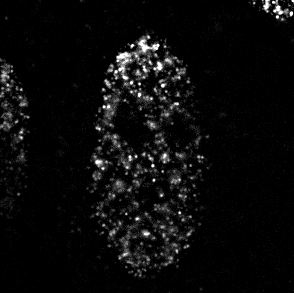
\includegraphics[scale=0.6]{/Users/cwseitz/git/cwseitz.github.io/docs/phd/ddpm/ddpm/media/Cell.png}
\caption{\textbf{Super-resolution of BRD4 in a HeLa cell}. (a) Immunofluorescence image of BRD4 labeled with Alexa488 secondary antibody. (b) Zoomed widefield image of the inset highlighted in red and the super-resolved image (SR) after application of an encoder $\phi$. (c) Multi-step photobleaching profile of the inset highlighted in blue.}
\end{figure}
